\pagestyle{empty}
\chapter*{\centering \large DAFTAR RIWAYAT HIDUP}
\thispagestyle{empty}

\begin{wrapfigure}{l}{4cm}
	\vspace{-25pt}
	\begin{center}
		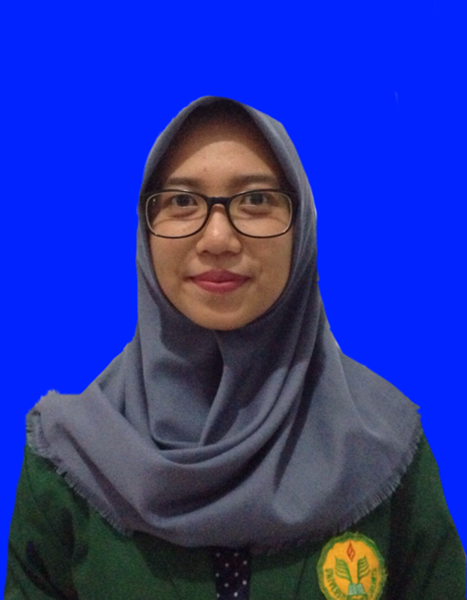
\includegraphics[width=0.27\textwidth]{gambar/pas-foto}
	\end{center}
	\vspace{-80pt}
\end{wrapfigure}

\noindent \textbf{MUHAMMAD YAN HANDOKO.}  Lahir di Semarang, 18 Juni 1997.  Anak pertama dari pasangan Bapak Muhammad dan Ibu Siti Wafirotun. Saat ini beralamatkan di Jl. Pengadegan Barat V RT.011 RW.007 No.18, Pancoran Jakarta Selatan.

\vspace{0.5cm}
\noindent
\begin{center}
	\begin{flushright}
		\begin{tabular}{lcl}
			No. Ponsel	& :&  082124022340 \\
			Email	& :&  myanhandkoko17@gmail.com
		\end{tabular}
	\end{flushright}
\end{center}
\vspace{0.5cm}

\noindent \textbf{Riwayat Pendidikan} : Penulis mengawali pendidikan di SDN Pengadegan 08 Pengadegan Pagi pada tahun 2002 - 2008. Setelah itu, penulis melanjutkan studi ke SMPN 154 Jakarta hingga tahun 2011. Kemudian melanjutkan ke SMAN 43 Jakarta pada tahun 2011-2014. Di Tahun 2014 penulis melanjutkan ke Universitas Negeri Jakarta (UNJ), Program Studi Ilmu Komputer, melalui jalur PENMABA. Di awal tahun 2019 (Senin, 18 Februari 2019) penulis telah memperoleh gelar Sarjana Komputer (S.Kom), Program Studi Ilmu Komputer, Fakultas Matematika dan Ilmu Pengetahuan Alam, Universitas Negeri Jakarta.

\noindent \textbf{Riwayat Organisasi} : Selama di bangku perkuliahan, penulis aktif di Badan Eksekutif Mahasiswa Jurusan Matematika sebagai staff Departemen Kaderisasi periode 2015-2016, Badan Eksekutif Mahasiswa Rumpun Matematika sebagai Ketua periode 2016-2017, Badan Eksekutif Mahasiswa Fakultas Matematika dan Ilmu Pengetahuan Alam sebagai Ketua periode 2017-2018, dan Badan Eksekutif Mahasiswa Universitas Negeri Jakarta sebagai Kepala Departemen Kaderisasi periode 2018. Penulis juga berpartisipasi dalam organisasi keilmiahan di Program Studi Ilmu Komputer yaitu DEFAULT, dimana penulis tergabung sebagai anggota divisi \textit{web}. Penulis juga tergabung dengan organisasi kemahasiswaan lain seperti, Masjid Ulul Albaab sebagai staff MUA \textit{Media Center} periode 2015, Desa Binaan FMIPA UNJ sebagai pengajar periode 2015-2016 dan kepala divisi informasi dan komunikasi periode 2015-2016, Tim Aksinya Kampus MIPA sebagai staff pusat pergerakan periode 2016-2017. Penulis juga kerap mengikuti kepanitiaan kegiatan yang diadakan oleh lembaga eksekutif (BEM), lembaga legislatif (LLM), dan lembaga dakwah fakultas (MUA), dan komunitas/\textit{underbow} lembaga (Default, Desa Binaan, TAnK MIPA). 